\section{Gesamtkonzept}

Aus den morphologischen Kasten und den Nutzwertanalysen wurde folgendes Gesamtkonzept ermittelt. 

\begin{figure}[H]
\centering
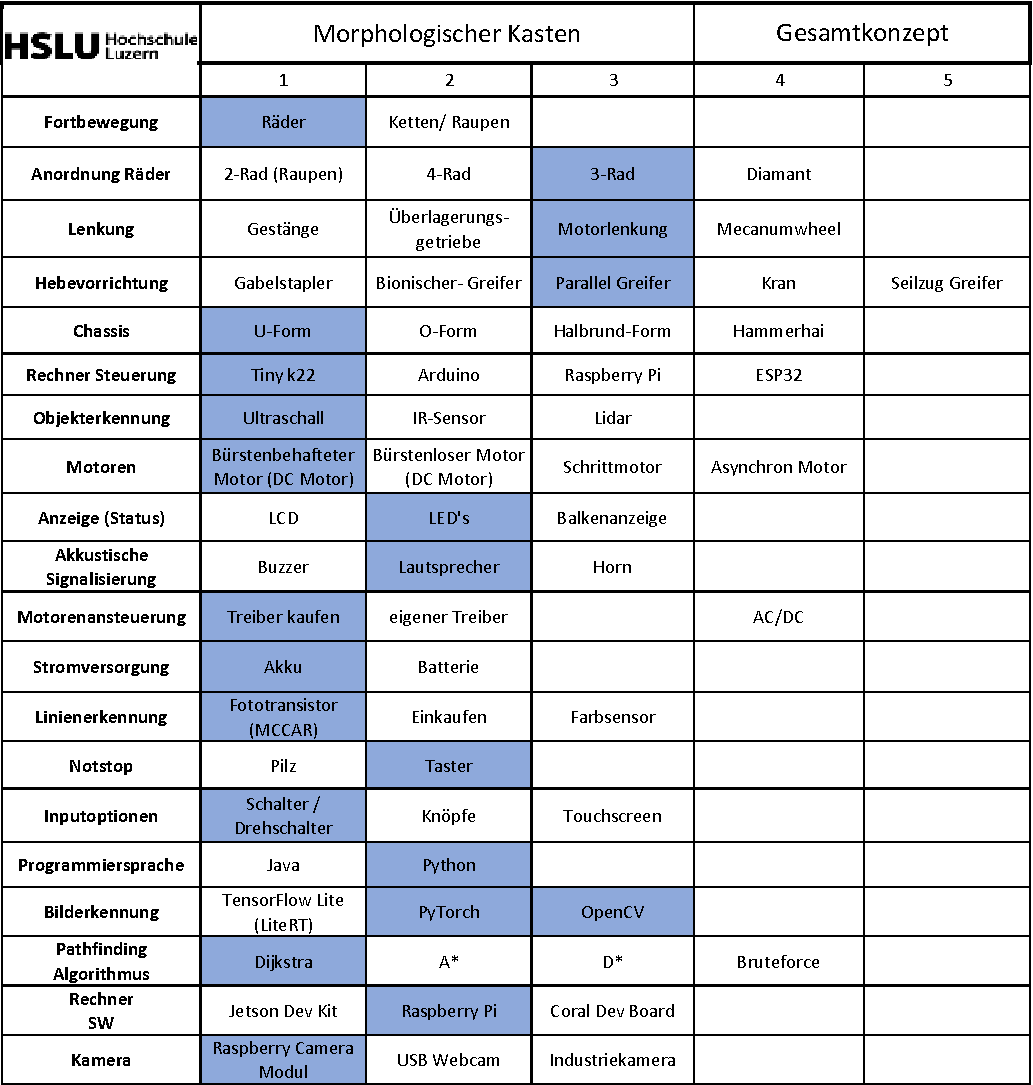
\includegraphics[width=\textwidth]{assets/MK-Gesamt.pdf}
\caption{Morphologischer Kasten}
\label{fig:mk-all}
\end{figure}

Es ist geplant einen Roboter in U-Form zu bauen, der sich mit drei Raedern fortbewegt und eine Motorlenkung besetzt. Hindernisse kann der Roboter mit einem Parallelgreifer anheben.

Die Steuerung wird auf einem Tiny k22 laufen. Die Distanz zu den Objekten werden mit Ultraschall erkannt und es wird ein buerstebehafteter Motor verwendet. Dieser Motor wird mit einem gekauften Treiber angesteuert. Die Stromversorgung laeuft ueber einen Akku. Der Akkustand und der Status des Roboters wird mit einem LED angezeigt. Damit der Roboter die Linien erkennt, wird ein Fototransistor verwendet. Das Ziel wird ueber einen Schalte von uns eingegeben.
Wenn der Roboter das Ziel erreicht, verkuendet er dies ueber einen Lautsprecher. Im Notfall wird der Roboter ueber einen Taster ausgeschaltet.

Die Software wird in Python geschrieben und laeuft auf einem Raspberry Pi.

\subsection{Schnittstellen}

PLACEHOLDER

\subsection{Ablauf}

PLACEHOLDER